\section{Evaluation}

Overall, our data set contains 233,538 samples that were collected from five volunteers. Each sample was collected every three seconds from a Microsoft Band smartwatch by our Android data collection system. In this section, we evaluate the performance of a few machine learning models on our dataset. We use some standard performance measures for our evaluation: precision, recall, and F1-score, for the classification models; RMSE and R$^2$ for the regression models. All reported performance values are determined via 5-fold cross-validation.

\subsection{Classification}

We want to warn a person if they are close to reaching the legal limit of 0.08 BAC. A good time to warn a user is at about 0.065 BAC. Using this threshold, the classes are split into 64\% is \textit{DRUNK}, and 36\% \textit{SOBER}.

To get a baseline, we first trained a logistic regression model. This model outputs values from 0.0 to 1.0, so we need to determine where to best split this output into each class. In Figure \ref{fig:log_pred_density}, we show a plot of the predictions of the model on the test data, using the actual labels to distinguish the output. \begin{figure}
	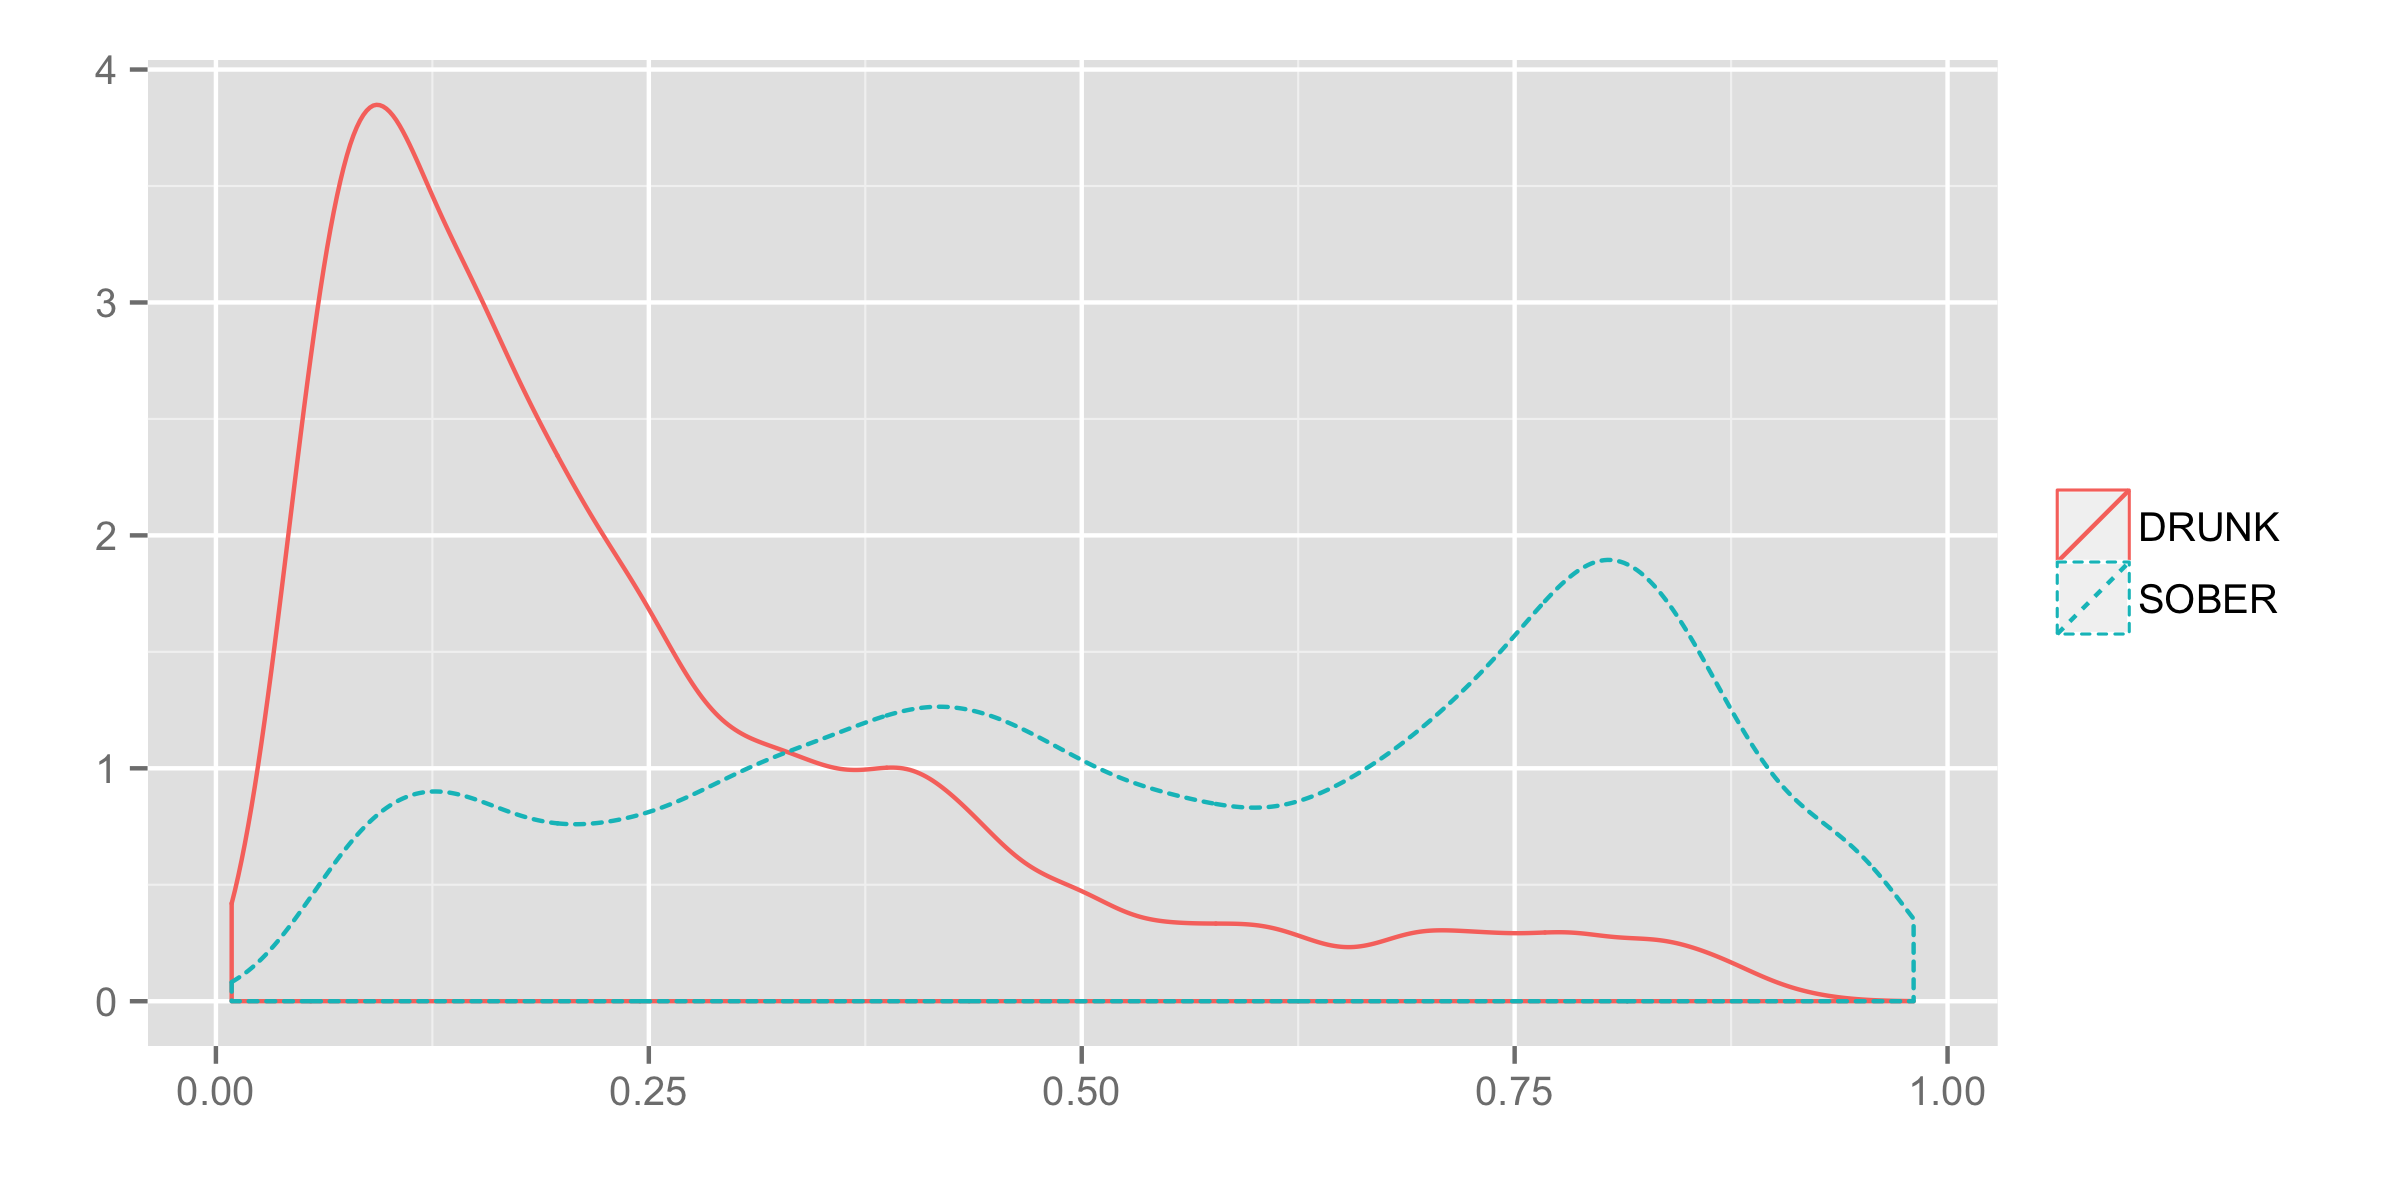
\includegraphics[width=1.0\textwidth]{../figs/log_pred_density}
	\caption{Logistic regression output frequency with actual labels.}
	\label{fig:log_pred_density}
\end{figure}In this plot, we see that the best threshold value for the logistic model predictions is around 0.32; above that we classify \textit{SOBER} and below that \textit{DRUNK}. Using this, we achieved a precision of 0.855 $\pm$ 0.002, recall of 0.730 $\pm$ 0.004, and F1-score of 0.787 $\pm$ 0.003.

Moving forward, we trained a SVM model using the Gaussian Radial Basis Function (RBF) kernel. For time constraints, the dataset was reduced by half using a uniform subsample. Even so, we found the SVM was able to achieve great performance with a precision of 0.886 $\pm$ 0.002, recall of 0.930 $\pm$ 0.002, and overall F1-score of 0.907 $\pm$ 0.001. Ideally we do not want to warn our users that they are drunk when they are not actually drunk, so we want to try and optimize the model to be as precise as possible. By modifying the error weighting to train against false positive errors, the SVM model achieved a precision of 0.970 $\pm$ 0.002, with recall of 0.729 $\pm$ 0.003, and F1-score of 0.832 $\pm$ 0.002. Our recall dropped for a higher precision, which is a well-known tradeoff for this kind of tuning, but this is fine. We can set a threshold on our smartphone warning system that if at least a recall fraction of the samples from our smartwatch are classified as \textit{DRUNK}, then there is a precision chance that the user is actually at 0.065 BAC.

\subsection{Regression}

So how does this do as a regression problem? We first considered the most basic: a linear regression model. This did not perform well at all. We next trained a neural network (ANN) model on the data. \begin{figure}
	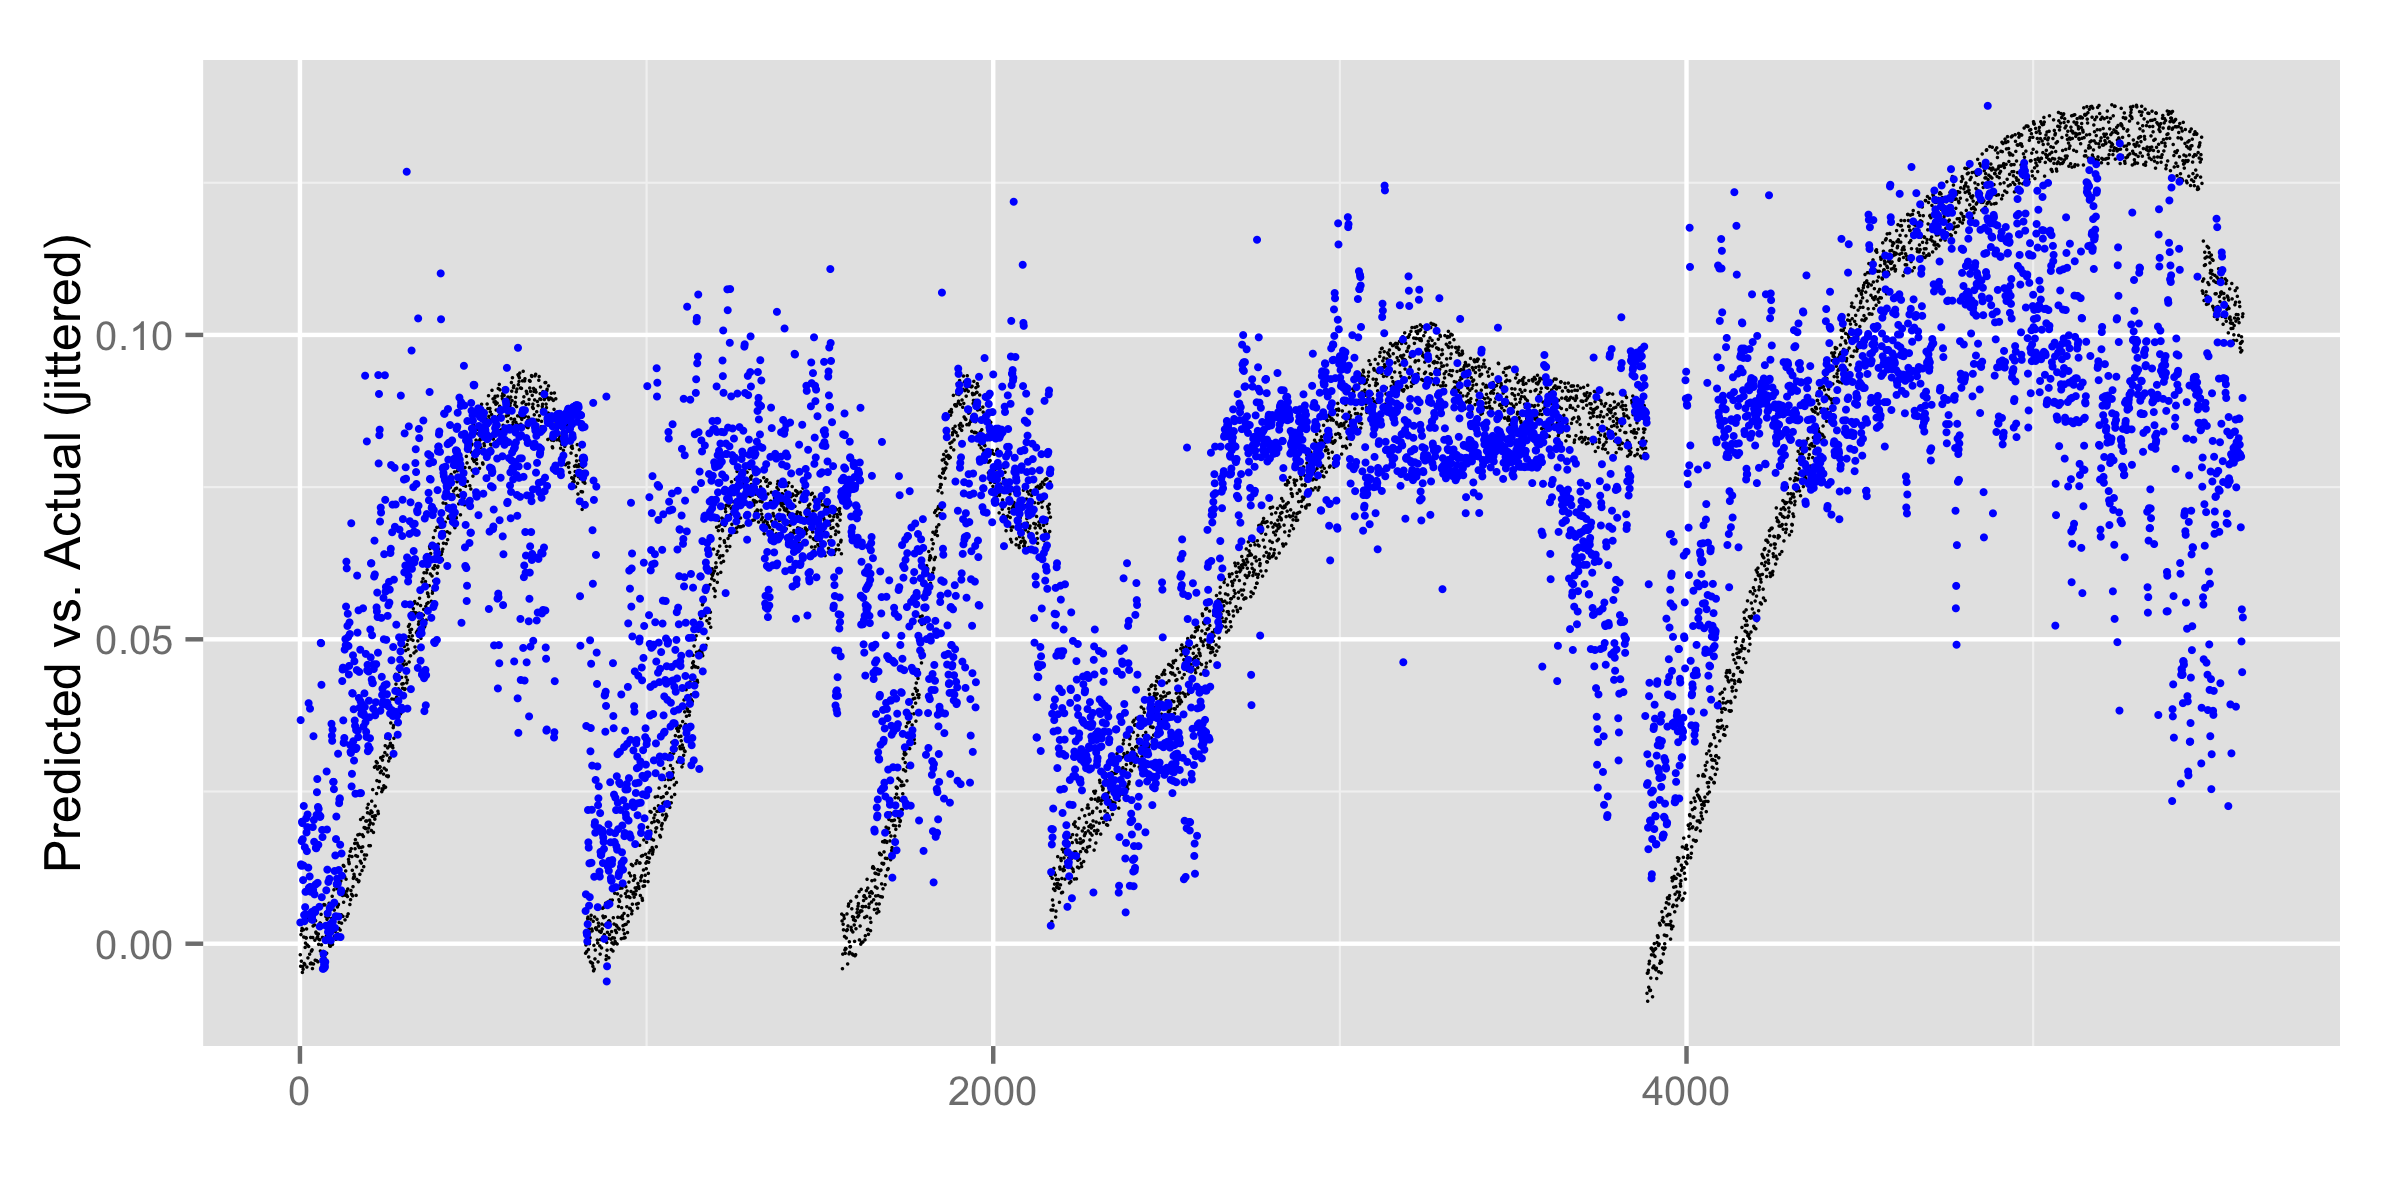
\includegraphics[width=1.0\textwidth]{../figs/nn_all}
	\caption{ANN predictions (blue) over actual BAC (black, jitterred) using test data.}
	\label{fig:nn_all}
\end{figure}This was even slower than the SVM which forced us to subsample to 8\% of the original data. The best performing ANN had a structure with two hidden layers of five nodes each. Figure \ref{fig:nn_all} plots the BAC predictions in of the neural network model on top of the actual values from the test set. The real values are jittered to give a sense of the density of the test data, the prediction values in blue are not. This model acheived a R$^2$ value of 0.525, with RMSE of 0.026. Much better than the linear regression model, but not nearly as good as the classification models.